\subsection{Influence of arm stiffness (Still relevant???)}
Several studies have shown that arm stiffness greatly influences the nature of movement. The stiffer the joints of the arm are, the easier it will be to control them. As reported in \cite{bennett1992time}, during cyclic tasks, the natural frequency of the human arm is adapted to match the first harmonic frequency. In human-robot systems, if the robot is not stiff enough, the system is highly unstable, leading the human to increase stiffness in his arm, thus creating even more instability. Hence, appropriate stiffness of the robotic arm is a paramount parameter for a successful interaction. This was demonstrated by studies showing that a system able to adapt its stiffness leads to smoother and more successful interactions. Based on that understanding, we postulate here, that stiffness also affects the ability of the arm to adapt to external stimulations and to learn new frequencies. 

\begin{figure}[h!]
\begin{center}
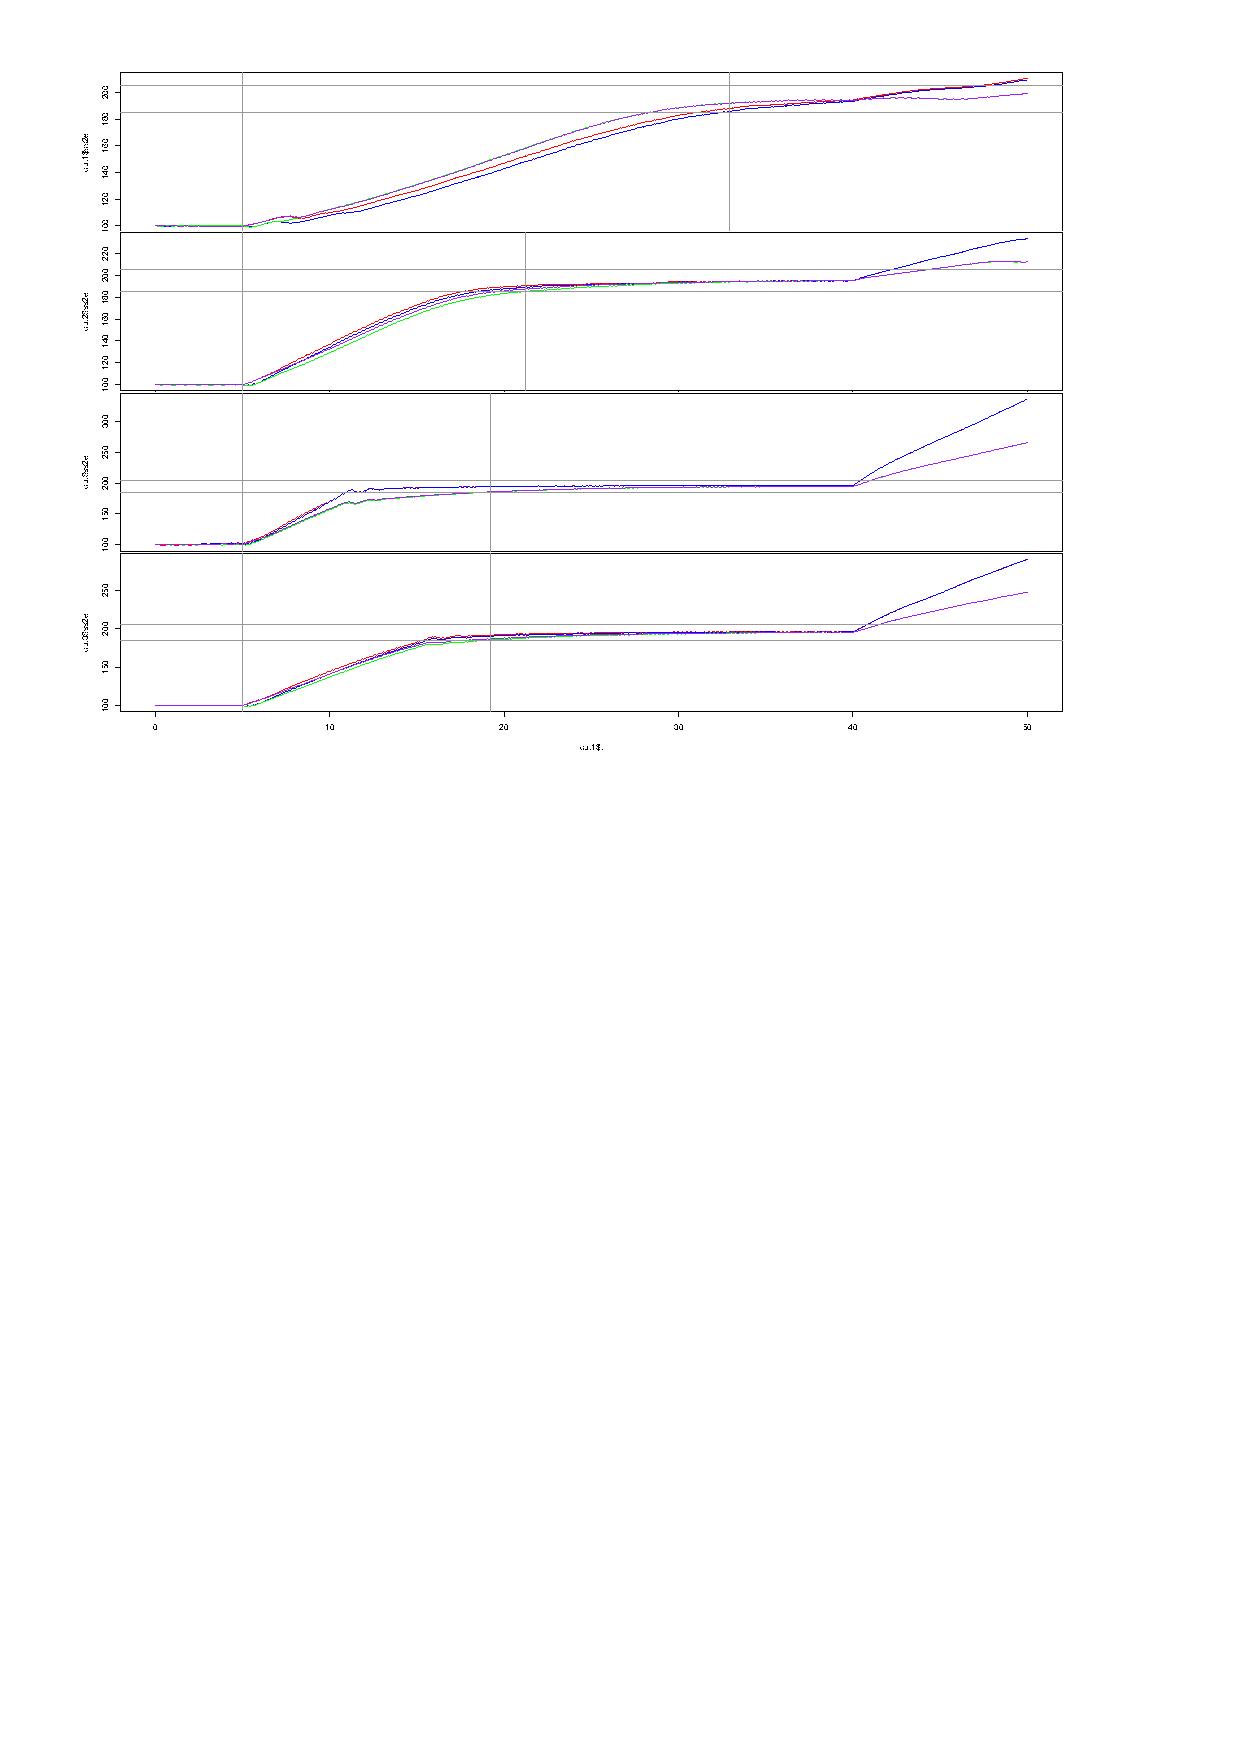
\includegraphics[width=10cm]{figures/simulation/varying_P}
\end{center}
\textbf{\refstepcounter{figure}\label{fig:20} Figure \arabic{figure}.} {Evolution of $\sigma_{S2E}$ and $\sigma_{S2F}$ for various values of P. For P = 1, response time is 16.2 s. For P = 0.01, response time is 27.9 s. For P = 0.08 and P = 0.1, response times are similar at 14.2.}
\end{figure}

\begin{figure}[h!]
\begin{center}
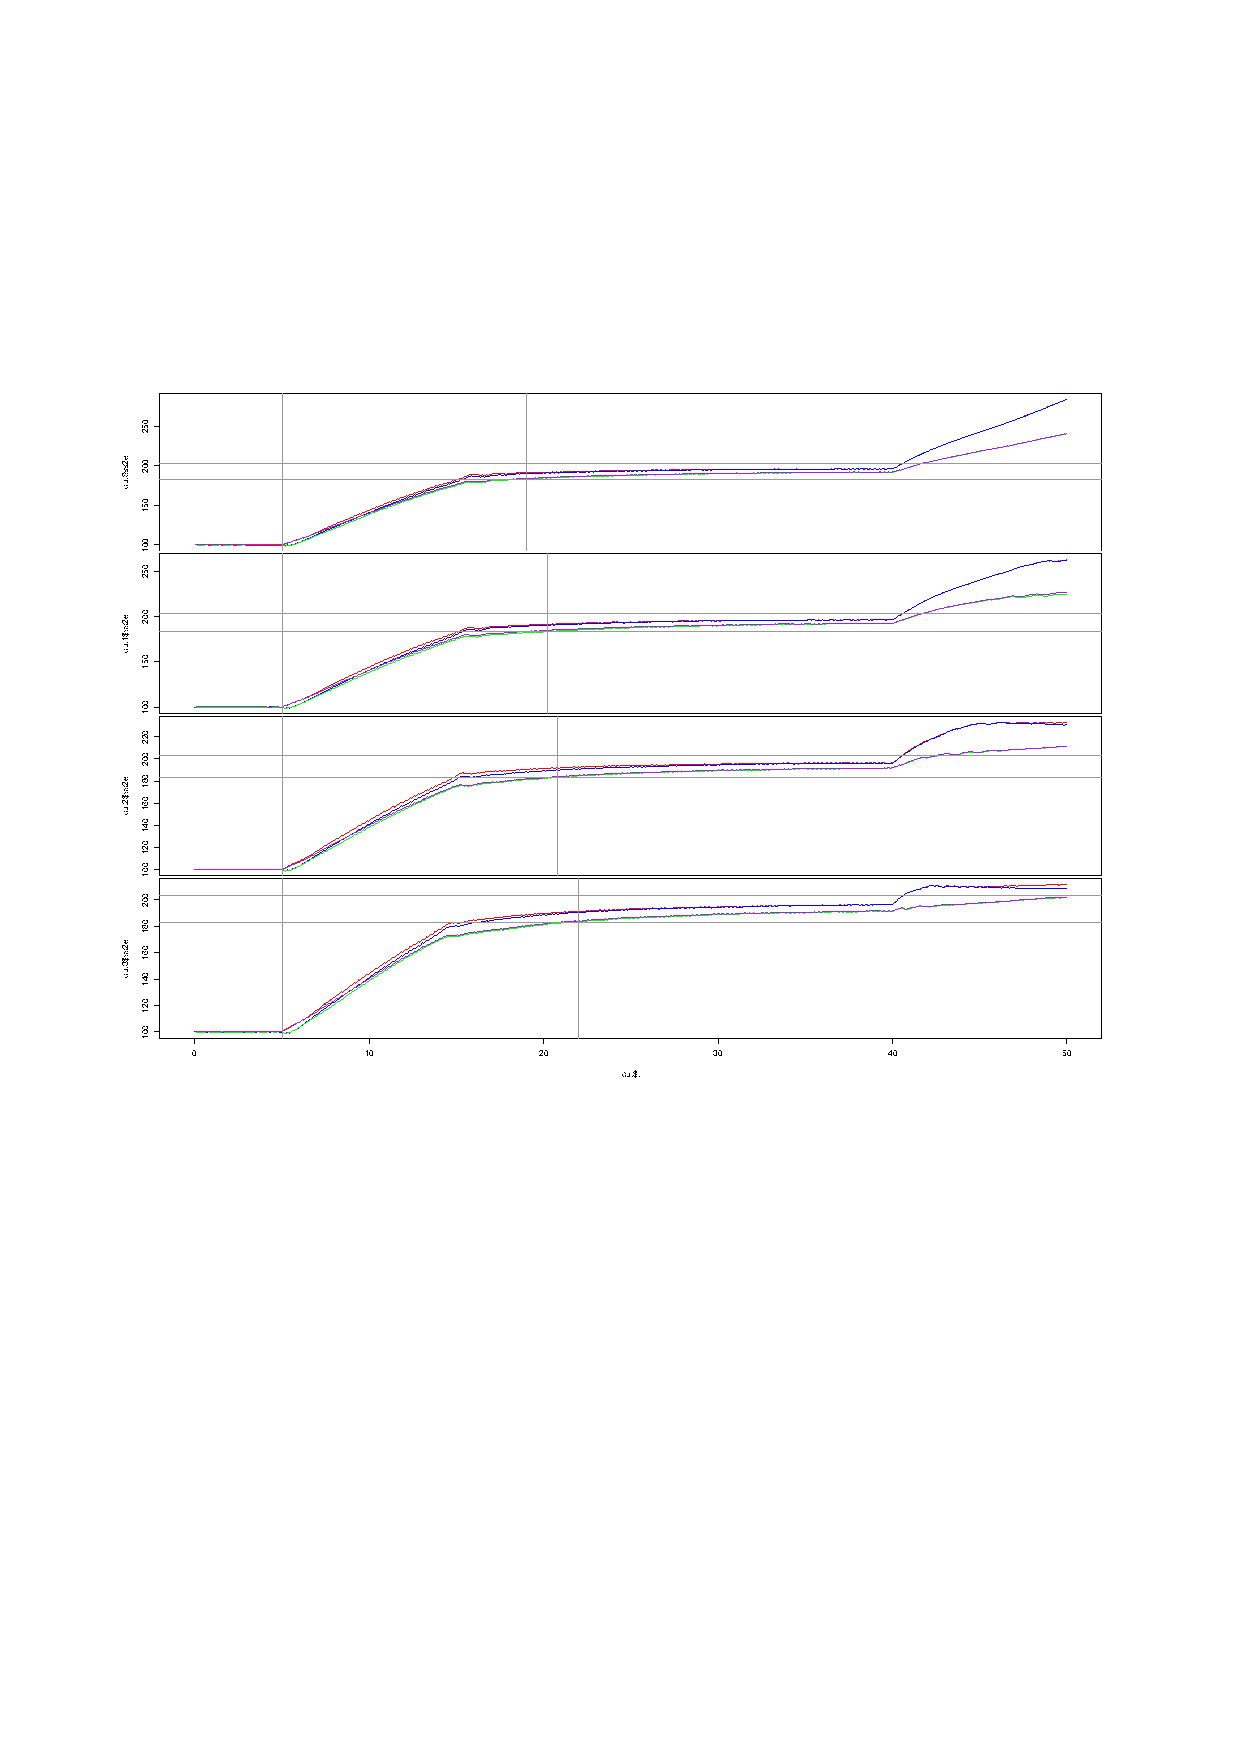
\includegraphics[width=10cm]{figures/simulation/varying_D}
\end{center}
 \textbf{\refstepcounter{figure}\label{fig:20} Figure \arabic{figure}.} {Evolution of $\sigma_{S2E}$ and $\sigma_{S2F}$ for various values of D (0, 0.0001, 0.0005 and 0.001). We can observe that the higher D is, the less the greater the system response is but the better it retains the learning of $\sigma_S$. For D = 0, response time is 14 s. For D = 0.0001, response time is 15.2 s. For D = 0.0005, response time is 15.8 s. For D = 0.001, response time is 17 s.}
\end{figure}

The evolution of $\sigma_S$ was recorded for various values of P and D. Varying P and D allows us to change the stiffness of the arm. It can be observed that P has indeed a strong influence on the response time of the system, ie. how fast it adapts to the new frequency. The higher P, the shorter the response time. But for P > 0.1, the arm becomes highly unstable and oscillates erratically before and during the interaction. On the contrary for D, the higher D, the longer the response time. We can also infer from our experiments that both parameters do influence how well the joint retains the learning.

\subsection{Experimental validation of the plastic CPG controlling the real robot}

\subsubsection{Protocol}
In this experimental setup, the robotic arm is at rest until a human perturbs it by initiating a handshaking movement (sinusoid in the vertical plane). When the interaction is over, the human releases the arm.
The parameters of the algorithm are the following: $\epsilon = 0.1$, $\tau_{m} = 0.5$, $\tau_{s} = 10.0$, $\tau_{r} = 0.005$, $W = 0.1$, $\sigma_{f} = 10.0$, $A_{f} = 1.0$. These parameters have been determined by running simulations beforehand to adapt well to the robot. When it is not mentioned, the PID constants for the robot are $P = 2.0$, $I = 0.0$, $D = 0.09$.

\subsubsection{Results}

In the first phase (before the interaction starts), the torque applied to the joint is zero. Hence, the motoneurons are perfectly in phase (see Figure 14) and the velocity sent to the joint is zero too. Subjected to no external influence, the system oscillates at its intrinsic frequency (see Figure 13). When the interaction starts, we can observe an increase in the force applied to the joints (30 N.m for both joints). The magnitude stays the same roughly 6 s. Then the force decreases and stays mainly stable at 15 N.m, this proves that the arm learned the movement. We can also observe from t = 12 onwards that F and v are synchronized. Finally the interaction stops and the human releases the robotic arm so there isn't any force exerted on the arm. We can see that the arm goes on oscillating at the frequency learned during the interaction, though with a much smaller amplitude.

\begin{figure}[h!]
\begin{center}
\includegraphics[width=15cm]{figures/cpg-coupled/F-s}
\end{center}
\textbf{\refstepcounter{figure}\label{fig:16} Figure \arabic{figure}.}{ Measure of torque and sent velocity for the second (left) and third (right) articulation during the experiment with the complete CPG. We can see that, during the first phase of the experiment, the robotic arm is not moving. It has not received any perturbation yet, so the motoneurons send the same signal, thus the difference between the two of them is zero. So the command sent to the robot is a zero speed. Right after the robot receives a perturbation, it starts oscillating and adapts to the human-imposed frequency. Once the arm is released, it goes on oscillating at the same frequency. This figure shows that the physical coupling between the human and the robot is achieved.}
\end{figure}

\begin{figure}[h!]
\begin{center}
\includegraphics[width=15cm]{figures/cpg-coupled/F-v}
\end{center}
\textbf{\refstepcounter{figure}\label{fig:16} Figure \arabic{figure}.}{ Measures of $V_{E}$ and torque for the second (left) and third (right) articulation during the experiment with the complete CPG. Here we can see the detailed phases of the experiment. We can see first the extensor cell oscillating at its intrinsic frequency. When the interaction begins, it adapts to the frequency of the torque. It is synchronized with the torque during the interaction, showing the robot has adapted. Finally, the frequency remains the same when the arm is released. It does not take into account the residual noise after the interaction. It shows that this algorithm makes the robot learn the right frequency.}
\end{figure}

\begin{figure}[h!]
\begin{center}
\includegraphics[width=15cm]{figures/cpg-coupled/v-pf-sn-mn}
\end{center}
\textbf{\refstepcounter{figure}\label{fig:18} Figure \arabic{figure}.}{ Evolution of the different cells with time during the same experiment, for both joints. We can see that the RG cells ($V$ on the figure) are in phase during the first phase of the experiment. This is because the robot has not interacted with the human yet. Then, the frequency adapts to the torque frequency and the two cells are in opposition of phase. Finally, when the arm is released, the two cells continue on being in opposition of phase. The pattern formation neurons are here to normalise the rhythm generator cells, and we can see that they follow the same pattern. The sensory neuron has to normalise the speed measured by the robot. Once again, the phases of the experiment appear clearly on this diagram. Finally, the last diagram shows the motoneurons output. We can see the two motoneurons do not have the same frequency during the interaction. This difference can be explained by the fact that we take two signals in opposition of phase from PF and we compare both of them against one signal coming from SN. The difference of phase between the two signals coming from PF explains the difference in amplitude for the motoneurons.}
\end{figure}

After a transitory phase, we can also observe that $\sigma_S$ and $\phi$ reach stability (see Figure 4). $\sigma_S$ stabilizes at a new value around 230 and we can infer from $\phi$ that both joints are in anti-phase. Finally the interaction stops, and $\sigma_S$ and phi remain stable at their new value. Thus proving that the CPG has indeed learned the new frequency.

\begin{figure}[h!]
\begin{center}
\includegraphics[width=15cm]{figures/cpg-coupled/ss-phi}
\end{center}
\textbf{\refstepcounter{figure}\label{fig:17} Figure \arabic{figure}.}{ On the left, evolution of $\sigma_{s}$ with time during the same experiment. This figure takes into account the four values of $\sigma_{s}$ that are present in the system: second joint extensor, second joint flexor, third joint extensor, third joint flexor. The four of them follow roughly the same direction, though some are ahead of the others at the start. The diagram shows the response time at 10\%, which is 11.97s. It is an acceptable response time for this interaction. We can even consider that the robot learned the frequency at around 11s (when $\sigma_{s}$ arrives to a plateau), which reduces the response time to 6s. The oscillations can also be affected by the human variability during the handshaking gesture, although, here, caution has been taken to remain homogeneous. When the interaction stops, all of the $\sigma_{s}$ values remain constant: the robot has learned the right frequency. 

On the right, evolution of $\phi$ (phase difference between the two joints) for the extensor and the flexor parts of the system. The two articulations are coupled in order to match the phase difference between the two corresponding joints on the human. It is an adaptation system based on the Righetti model, not a learning model (meaning that it adapts as long as the interaction is going, but when the interaction ends, the difference of phase diverges). The robot has adapted its phase difference roughly at the same time it has learned the frequency (with $\sigma_{s}$). We can see here that joint 2 is almost in opposition of phase with joint 3. Also, the phase difference in the flexor part is the same as the phase difference in the extensor part (modulo $2 \pi)$), which is to be expected.}
\end{figure}


\begin{figure}[h!]
\begin{center}
\includegraphics[width=15cm]{figures/cpg-coupled/dp}
\end{center}
\textbf{\refstepcounter{figure}\label{fig:19} Figure \arabic{figure}.}{ On the left, phase portrait of the arm movement for the second and third articulations, during the same experiment. Here we can only see two cycles. In fact, the first five seconds of the experiment are located at the starting point, since the robot does not move at all. The outer cycle is the interaction part, while the inner cycle is the "arm released" part. Once again, the cycle does not change in shape, but changes in size (due to the amplitude modification) when the arm is released. 
On the right, phase portrait in the $(V, y)$ plan for the second and third articulations, during the same experiment. Three different cycles can be seen here. First, the starting cycle (most inner circle on the four diagrams), when the rhythmic cells oscillate at their intrinsic frequency. Then, the interaction cycle (most outer circle) when the human and the robot are interacting. Finally, the middle circle is the end cycle: it has the same shape as the interaction cycle, but it changes in size. The fact that cycles appear show that the system is stable, meaning the frequency is learned.}
\end{figure}

\subsubsection{Influence of arm stiffness}

As with the simulation, the evolution of $\sigma_S$ was recorded for various values of P and D. Once more, varying P and D allows us to change the stiffness of the arm. It can be observed that P and D have indeed a strong influence on the response time of the system, ie. how fast it adapts to the new frequency. The higher P, the shorter the response time. Similarly for D, the higher D, the shorter the response time. 

The same observations were made on the simulated robot for P. But we can observe the contrary for D. For the robot, the greater D, the faster the system reacts. This can be explained by dissimilar implementations of the PID.

\begin{figure}[h!]
\begin{center}
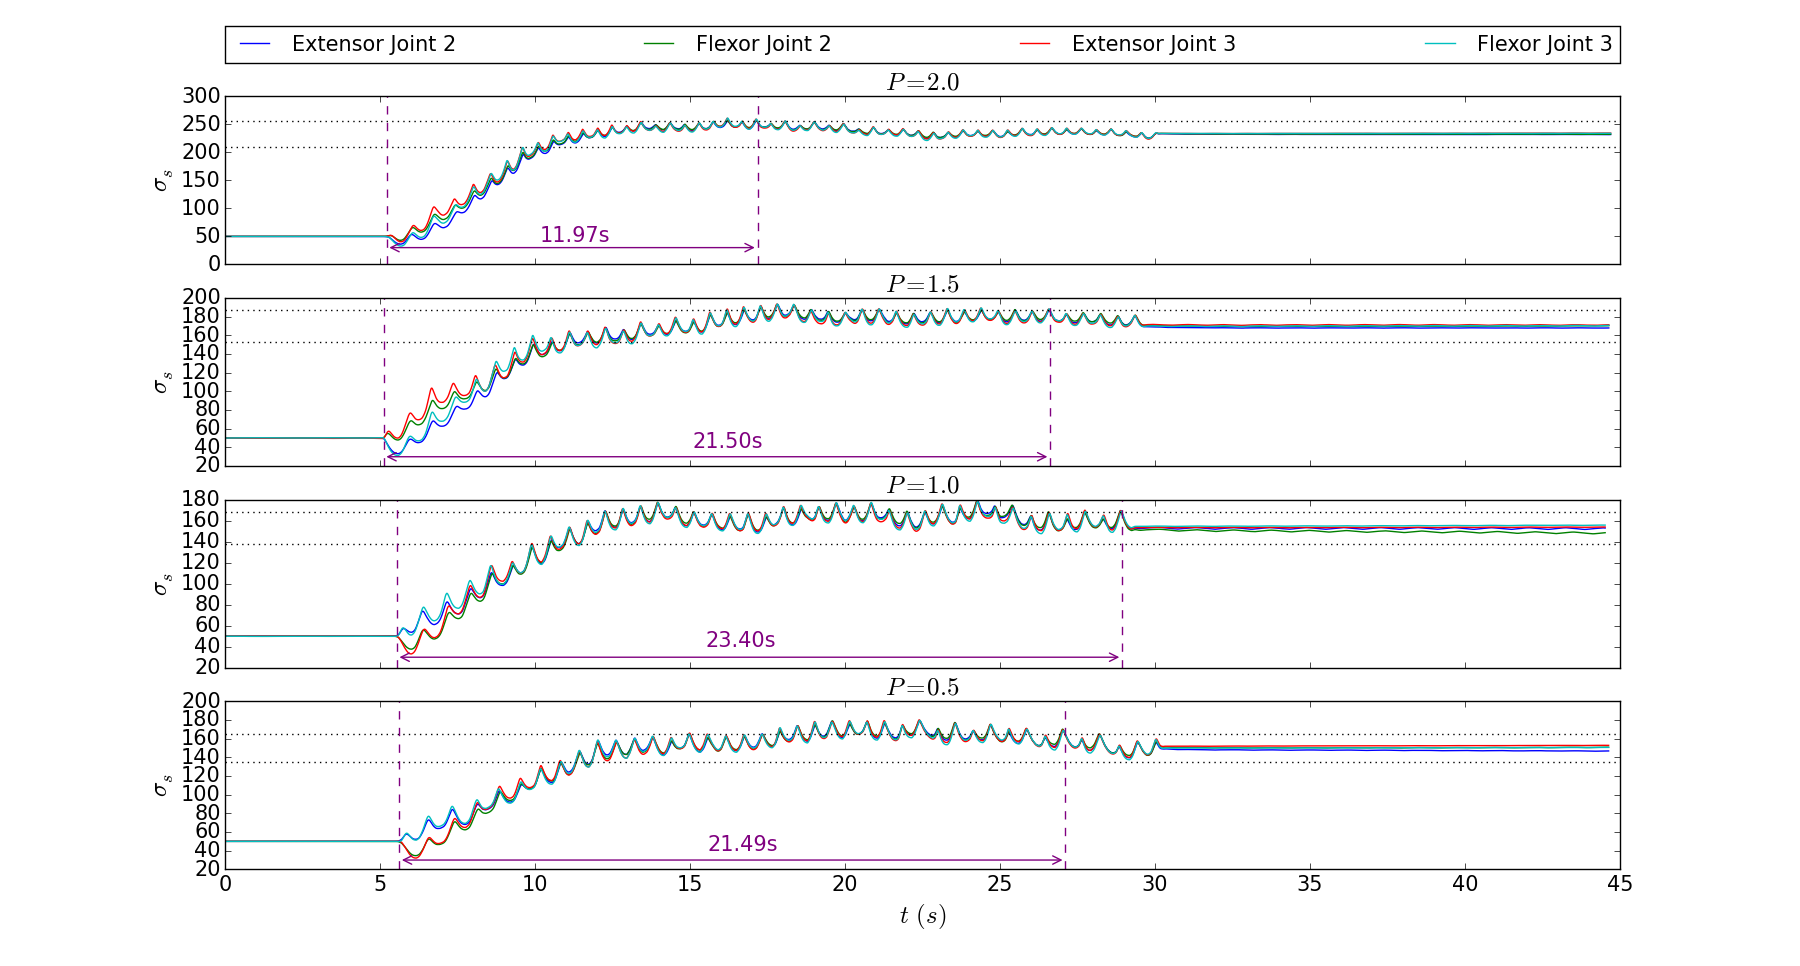
\includegraphics[width=10cm]{figures/cpg-coupled/PID-P}
\end{center}
\textbf{\refstepcounter{figure}\label{fig:20} Figure \arabic{figure}.}{ Influence of P in the learning process (the other values, I and D, are the default values, 0 and 0.05). We can clearly see that the greater the P, the faster the system is (its response time is reduced). It is to be expected, of course. Another interesting fact is that the final value of $\sigma_{s}$ decreases as P decreases: this means the robot arm cannot achieve high frequency values when P is too small. This is also to be expected, since the system takes more time to reach the target position.}
\end{figure}

\begin{figure}[h!]
\begin{center}
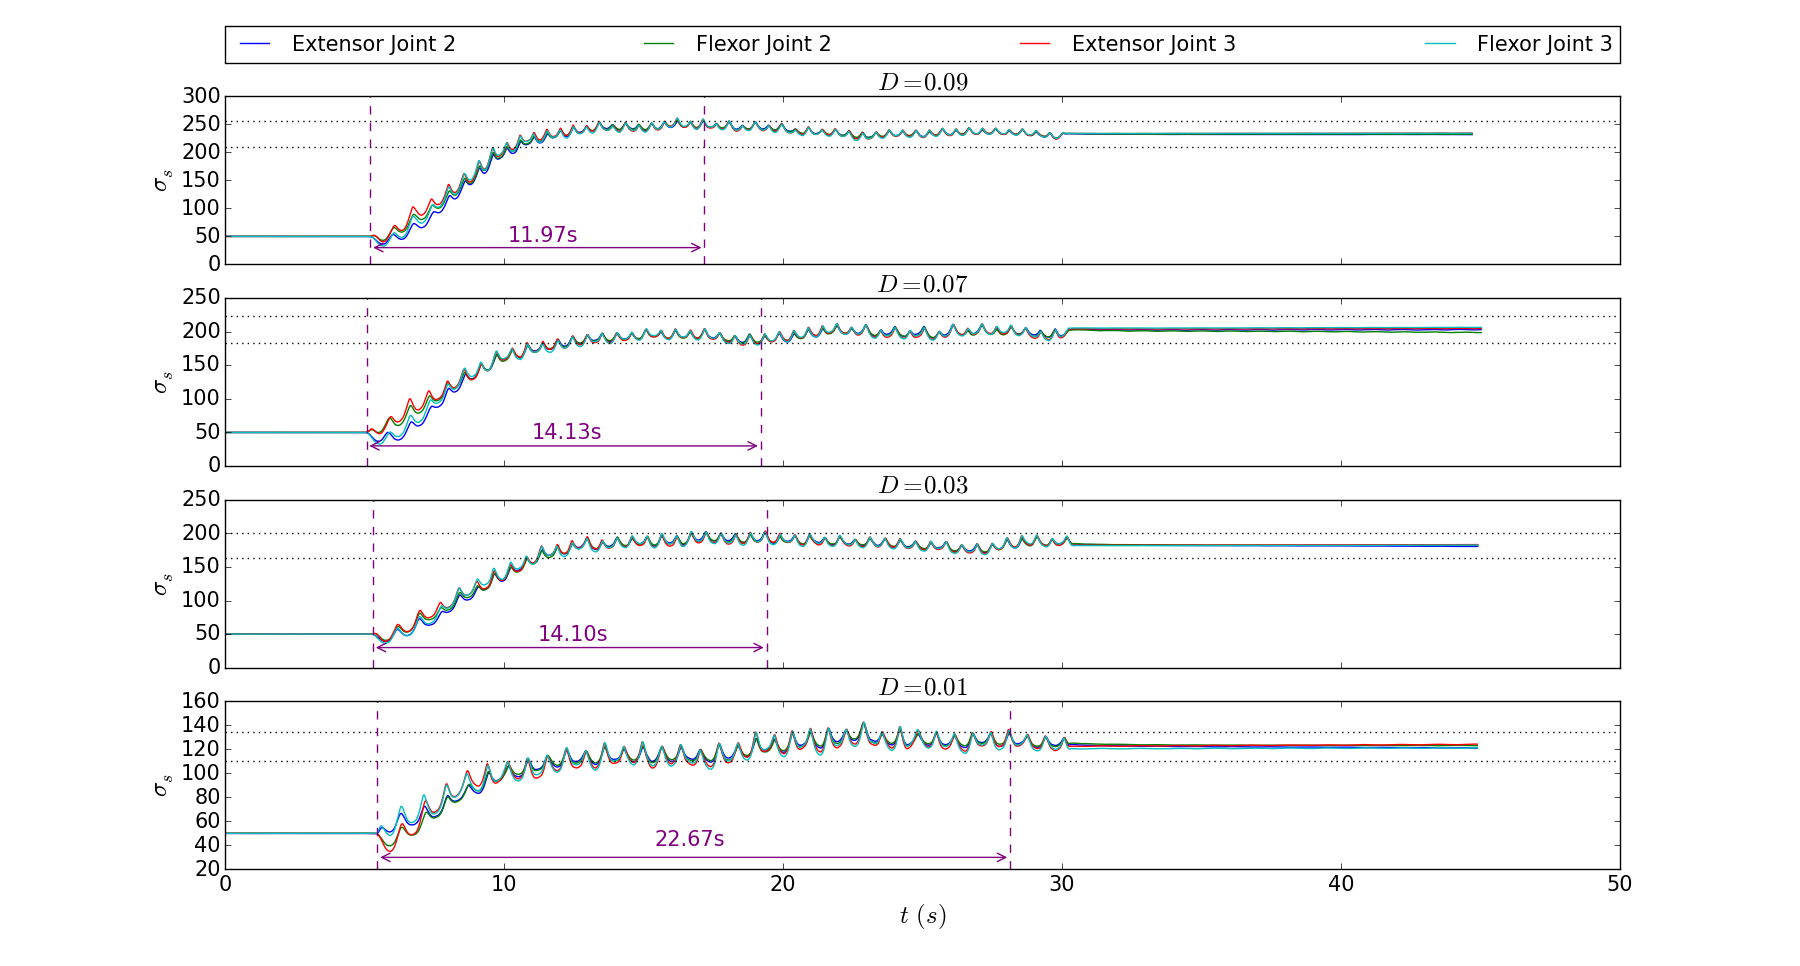
\includegraphics[width=10cm]{figures/cpg-coupled/PID-D}
\end{center}
\textbf{\refstepcounter{figure}\label{fig:20} Figure \arabic{figure}.}{ Influence of D in the learning process (the other values, P and D, are the default values, 2 and 0). We can make the same observations as with P, though the response time remains correct for D greater than 0.03. }
\end{figure}

The stability and speed of the algorithm are better when P and D are increased.

